\documentclass[UTF8,a4paper,11pt]{ctexart}

\usepackage{geometry}
\geometry{left=2.2cm,right=2.2cm,top=2.2cm,bottom=2.2cm}

\usepackage{booktabs}
\usepackage{array}
\usepackage{graphicx}
\usepackage{subcaption}
\usepackage{hyperref}
\usepackage{xcolor}

\graphicspath{{figures/}}

\title{K7 直播间短视频：数据预处理与分类验证报告}
\author{Yunxi}
\date{\today}

\begin{document}
\maketitle

\section{背景与目标}
本报告对应 \texttt{Week2\_Task.md} 的交付要求（Task3）。目标是基于已构建好的主表，对``爆款''与``非爆款''两组在核心绩效指标上的差异进行描述性统计与可视化，并给出对现有分类合理性的初步判断与疑问记录。

\section{数据资产与口径说明}
\subsection{输入数据}
\begin{itemize}
  \item 主表：\texttt{Processed\_Data/main\_perf\_merged\_all.xlsx}（由任务二产出，包含 \texttt{is\_popular} 标签与 \texttt{source} 来源字段）。
  \item 图表文件：\texttt{Deliverables/week2\_task3/figures/}（本报告插图直接引用该目录下 png）。
\end{itemize}

\subsection{分组字段与样本规模}
分组字段为 \texttt{is\_popular}（0=非爆款，1=爆款）。基于主表统计：
\begin{itemize}
  \item 总样本量：13856 条；
  \item 爆款：1895 条（13.68\%）；
  \item 非爆款：11961 条（86.32\%）。
\end{itemize}
按数据来源 \texttt{source} 分层（dy/k7）统计如下：
\begin{center}
\begin{tabular}{lrr}
\toprule
source & 非爆款 & 爆款 \\
\midrule
dy & 10786 & 1752 \\
k7 & 1175 & 143 \\
\bottomrule
\end{tabular}
\end{center}

\section{数据清洗、对齐与整合方法（任务一/二回顾）}
本节描述了数据清洗、对齐、整合的具体过程与方法，细节实现与过程记录见：


\texttt{Analysis/Week2\_Task1.ipynb}、\texttt{Analysis/Week2\_Task2.ipynb}。

\subsection{多源对齐与合并}
\begin{itemize}
  \item 对齐对象：K7 视频素材报表与金运抖音每日绩效数据。
  \item 对齐方式：以素材/视频的唯一标识（如素材ID、文件名规范化后的匹配键）进行匹配；对每日绩效数据做多日合并，形成可按素材维度分析的主表。
  \item 合并策略：构建 \texttt{merged\_common}（两批数据共有字段）与 \texttt{merged\_all}（尽可能保留全量字段），并保留 \texttt{source} 以区分 dy/k7。
\end{itemize}

\subsection{异常与缺失处理}
\begin{itemize}
  \item 缺失值：对关键指标列进行数值化与缺失处理（空值保留为 NA，在统计与绘图阶段按指标列 dropna）。
  \item 异常值：对``率''类指标中过大异常（例如 >100）样本进行过滤，以避免口径错误/抓取异常导致统计偏移（具体阈值与过滤实现见任务二 notebook）。
  \item 字段统一：对不同数据源同义字段进行统一命名（例如整体消耗/基础消耗归并、点击率/转化率字段统一）。
\end{itemize}

\subsection{业务特征整合（可用属性）}
\begin{itemize}
  \item 时间特征：补充节假日、星期、月份等派生字段。
  \item 文本特征：对标题进行规范化；在可用情况下整合 LLM/embedding 等衍生字段（用于后续更深入的内容侧分析）。
\end{itemize}

\section{爆款标签构建与验证策略}
\subsection{现有标签说明}
任务二中为保证 dy 与 k7 两批素材使用统一口径，采用以下规则生成 \texttt{is\_popular}：
\begin{itemize}
  \item 以 \texttt{消耗} 的箱线图上边界（Q3 + 1.5IQR）刻画``高流量/高投放''样本；
  \item 在高消耗样本中，要求 \texttt{点击率} 或 \texttt{转化率} 至少一个达到上四分位（Q3），以刻画``效率''；
  \item 满足上述条件则标为爆款，否则为非爆款。
\end{itemize}

\subsection{验证原则}
由于 \texttt{is\_popular} 的生成直接使用了 \texttt{消耗/点击率/转化率}，因此这三个指标在两组上的差异属于规则内生，更适合作为口径解释而非验证证据。

因此本报告的分类验证优先查看未直接参与打标的指标：播放与互动、直播间行为、成交相关指标（可视作 GMV/订单代理指标）等。

\section{描述性统计对比结果（附表）}
表~\ref{tab:effect} 给出部分关键验证指标的对比摘要（非爆款 vs 爆款）。其中：
\begin{itemize}
  \item Median ratio 仅在非爆款中位数非 0 时可计算；
  \item 同时给出Mean ratio以反映长尾样本对均值的影响。
\end{itemize}

\begin{table}[h]
\centering
\caption{关键验证指标：爆款 vs 非爆款}
\label{tab:effect}
\begin{tabular}{lrrrr}
\toprule
指标 & Median(非爆款) & Median(爆款) & Median ratio & Mean ratio \\
\midrule
展示次数 & 95 & 31126 & 327.642 & 15.442 \\
播放数 & 74 & 31928 & 431.459 & 15.440 \\
有效播放数 & 23 & 7193 & 312.739 & 19.417 \\
点击次数 & 6 & 1459.5 & 243.250 & 12.666 \\
转化数 & 0 & 37 & -- & 24.594 \\
直接成交金额 & 0 & 6373.6 & -- & 24.803 \\
直接支付ROI & 0 & 2.67 & -- & 2.030 \\
直播间观看人次 & 10 & 1581 & 158.100 & 11.968 \\
\bottomrule
\end{tabular}
\end{table}

\textbf{初步观察：}
\begin{itemize}
  \item 在验证指标上，爆款组整体显著高于非爆款组（如播放、展示、成交金额、直播间观看等），说明现有分类与绩效表现大体一致；
  \item 多个指标的非爆款中位数为 0（例如成交金额、部分互动），说明数据整体呈现长尾分布，0值较多。
\end{itemize}

\section{可视化对比结果}
下列图表均已保存至 \texttt{Deliverables/week2\_task3/figures/}。

\begin{figure}[h]
  \centering
  \begin{subfigure}[t]{0.48\textwidth}
    \centering
    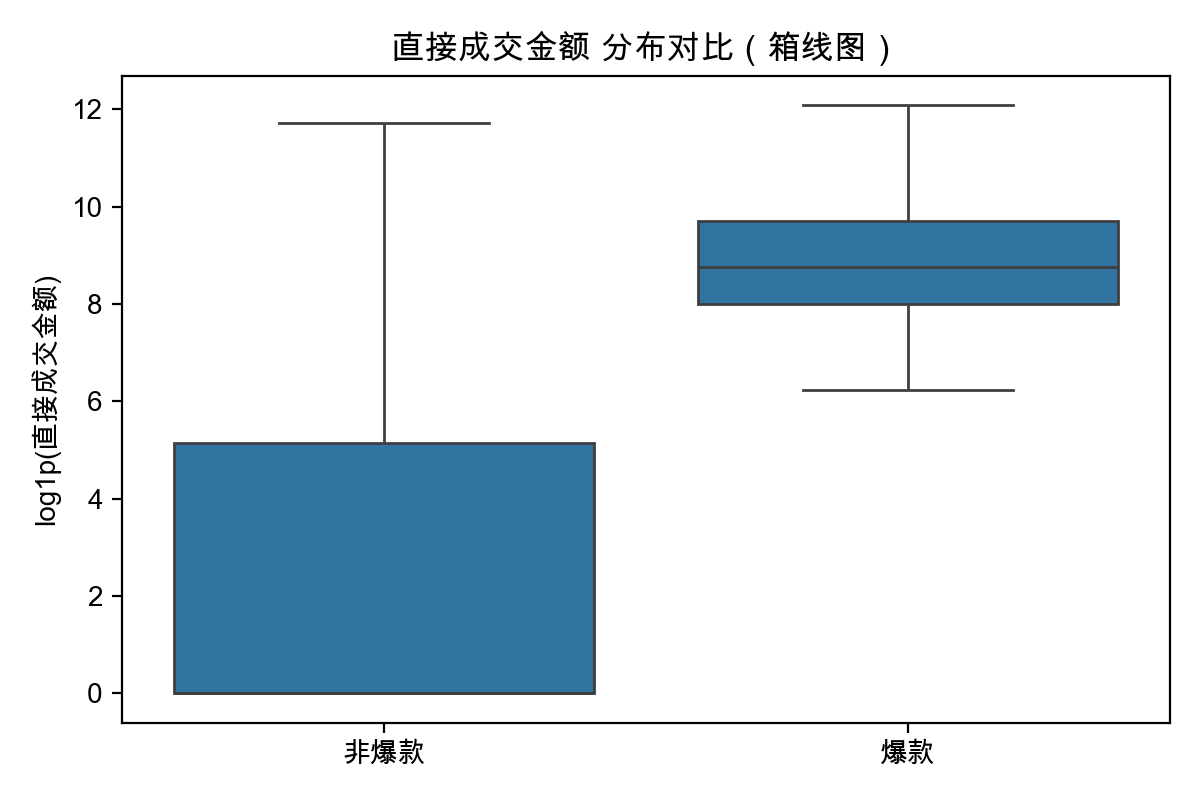
\includegraphics[width=\linewidth]{box_metric_3d0bc096.png}
    \caption{箱线图（log1p）}
  \end{subfigure}
  \hfill
  \begin{subfigure}[t]{0.48\textwidth}
    \centering
    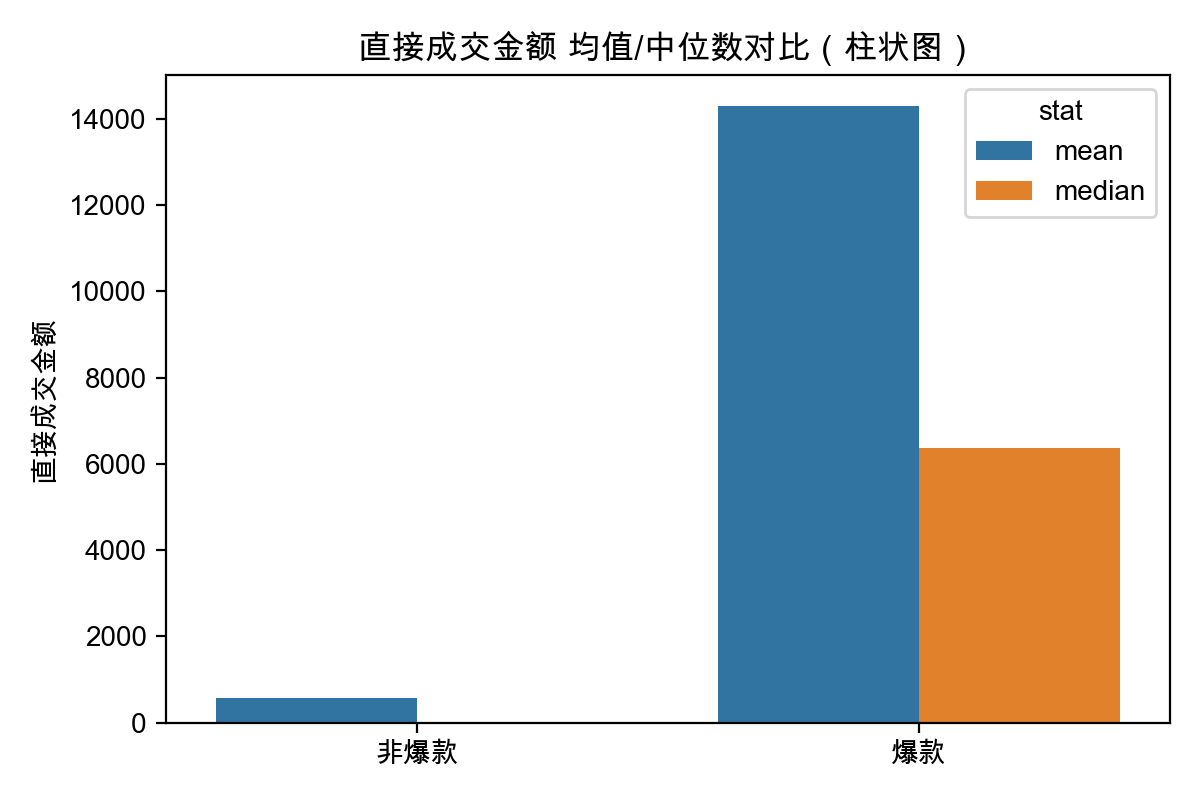
\includegraphics[width=\linewidth]{bar_metric_3d0bc096.png}
    \caption{柱状图（均值/中位数）}
  \end{subfigure}
  \caption{成交表现-直接成交金额：爆款 vs 非爆款}
\end{figure}

\begin{figure}[h]
  \centering
  \begin{subfigure}[t]{0.48\textwidth}
    \centering
    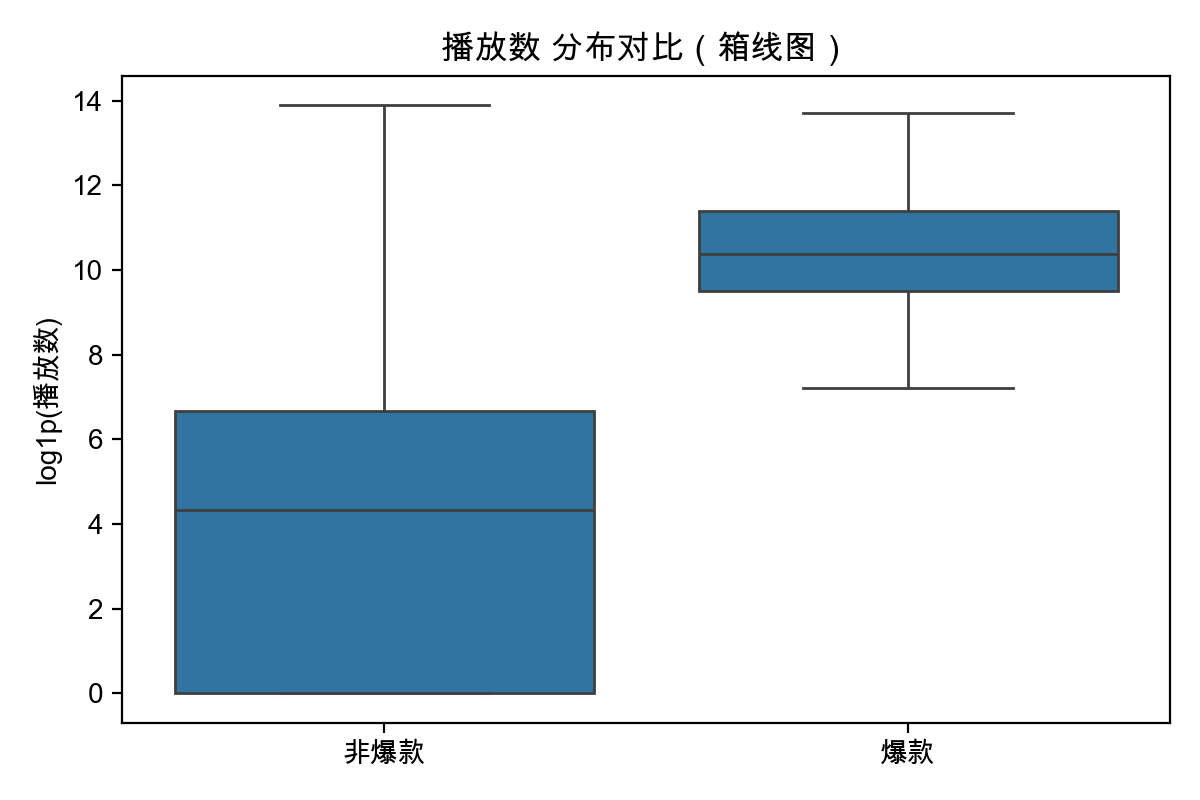
\includegraphics[width=\linewidth]{box_metric_b9302462.png}
    \caption{箱线图（log1p）}
  \end{subfigure}
  \hfill
  \begin{subfigure}[t]{0.48\textwidth}
    \centering
    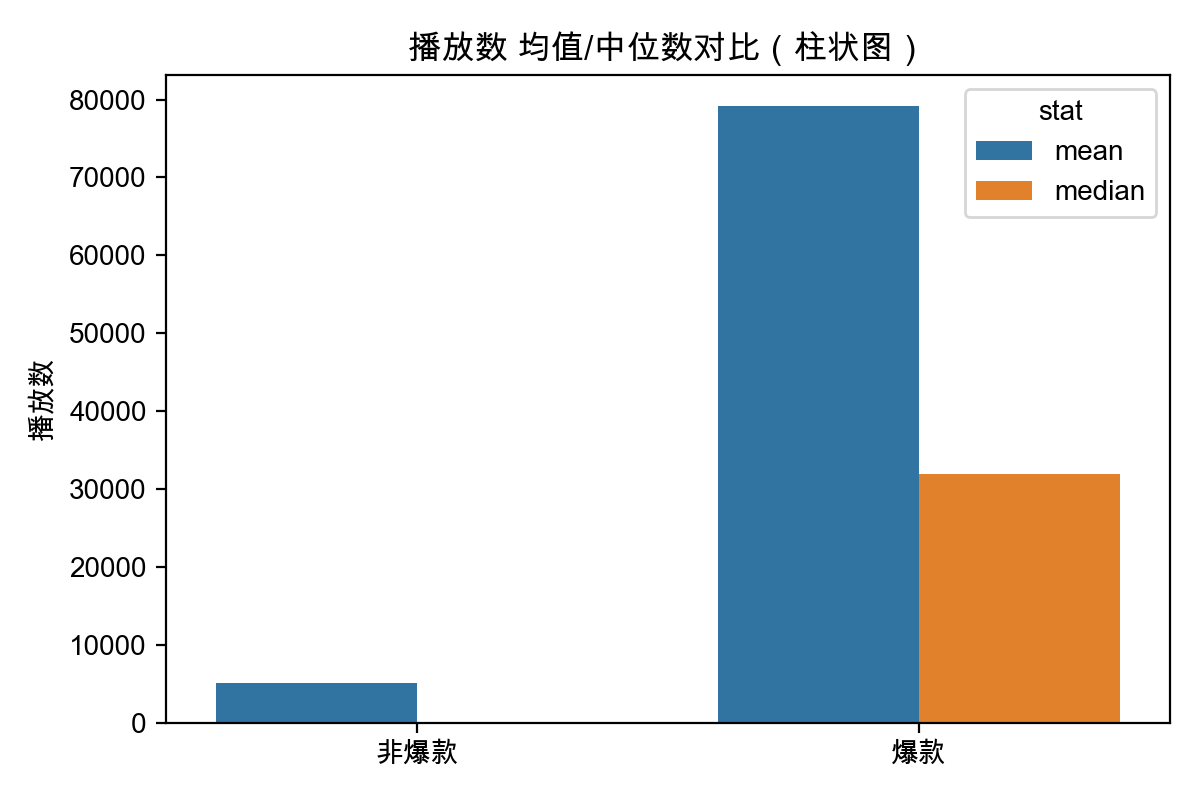
\includegraphics[width=\linewidth]{bar_metric_b9302462.png}
    \caption{柱状图（均值/中位数）}
  \end{subfigure}
  \caption{内容传播-播放数：爆款 vs 非爆款}
\end{figure}


\begin{figure}[h]
  \centering
  \begin{subfigure}[t]{0.48\textwidth}
    \centering
    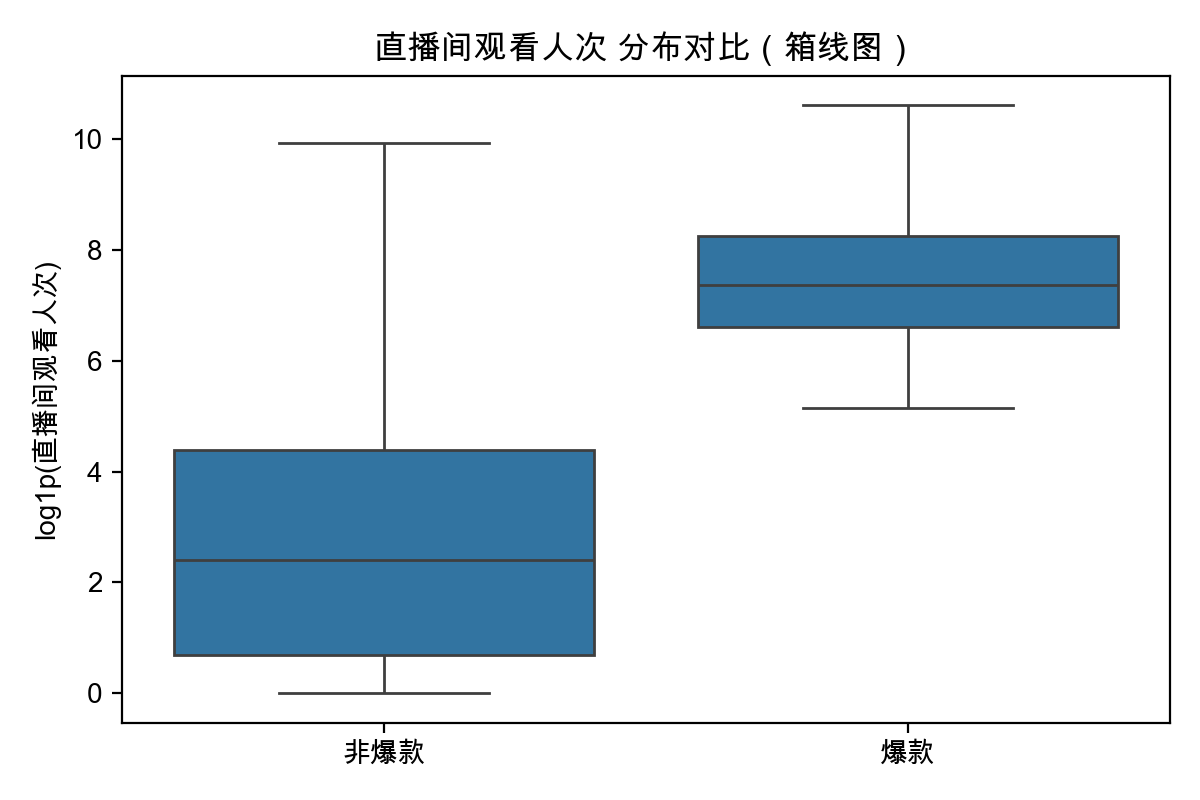
\includegraphics[width=\linewidth]{box_metric_b7fbac10.png}
    \caption{箱线图（log1p）}
  \end{subfigure}
  \hfill
  \begin{subfigure}[t]{0.48\textwidth}
    \centering
    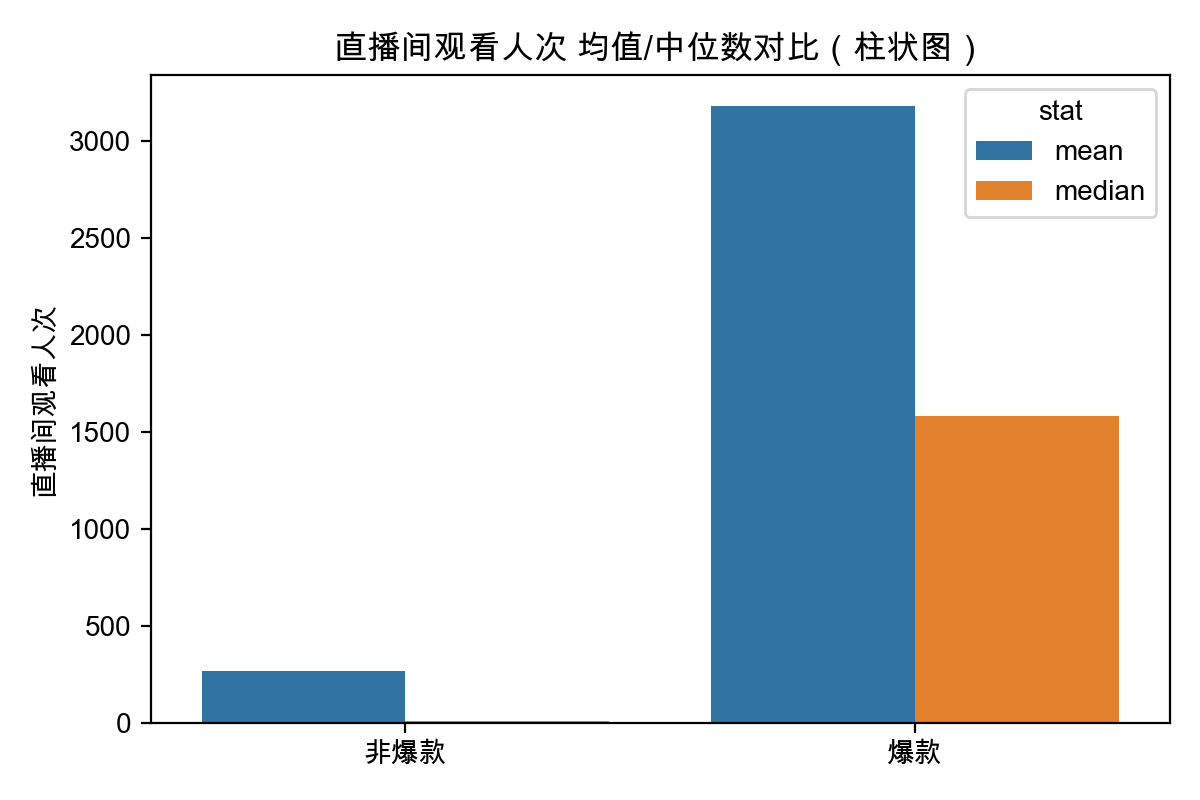
\includegraphics[width=\linewidth]{bar_metric_b7fbac10.png}
    \caption{柱状图（均值/中位数）}
  \end{subfigure}
  \caption{直播间行为-直播间观看人次：爆款 vs 非爆款}
\end{figure}

\begin{figure}[h]
  \centering
  \begin{subfigure}[t]{0.48\textwidth}
    \centering
    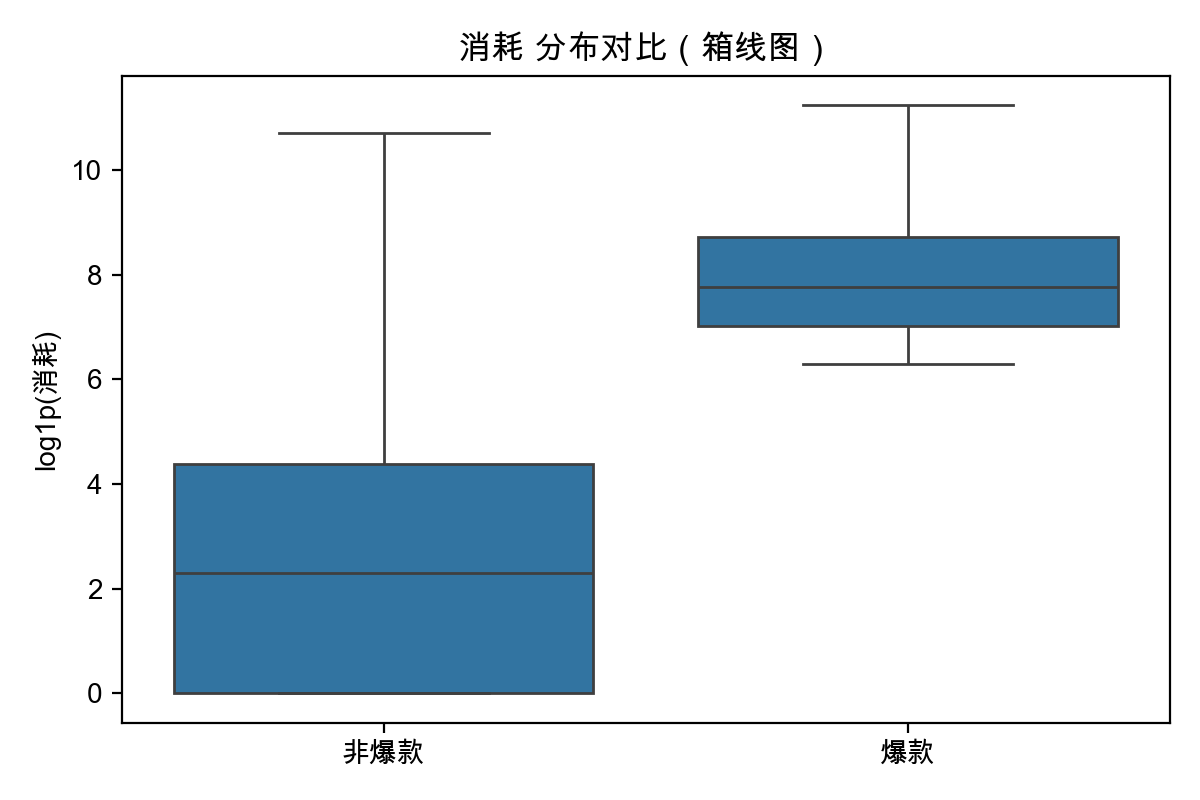
\includegraphics[width=\linewidth]{box_metric_4ab855fb.png}
    \caption{箱线图（log1p）}
  \end{subfigure}
  \hfill
  \begin{subfigure}[t]{0.48\textwidth}
    \centering
    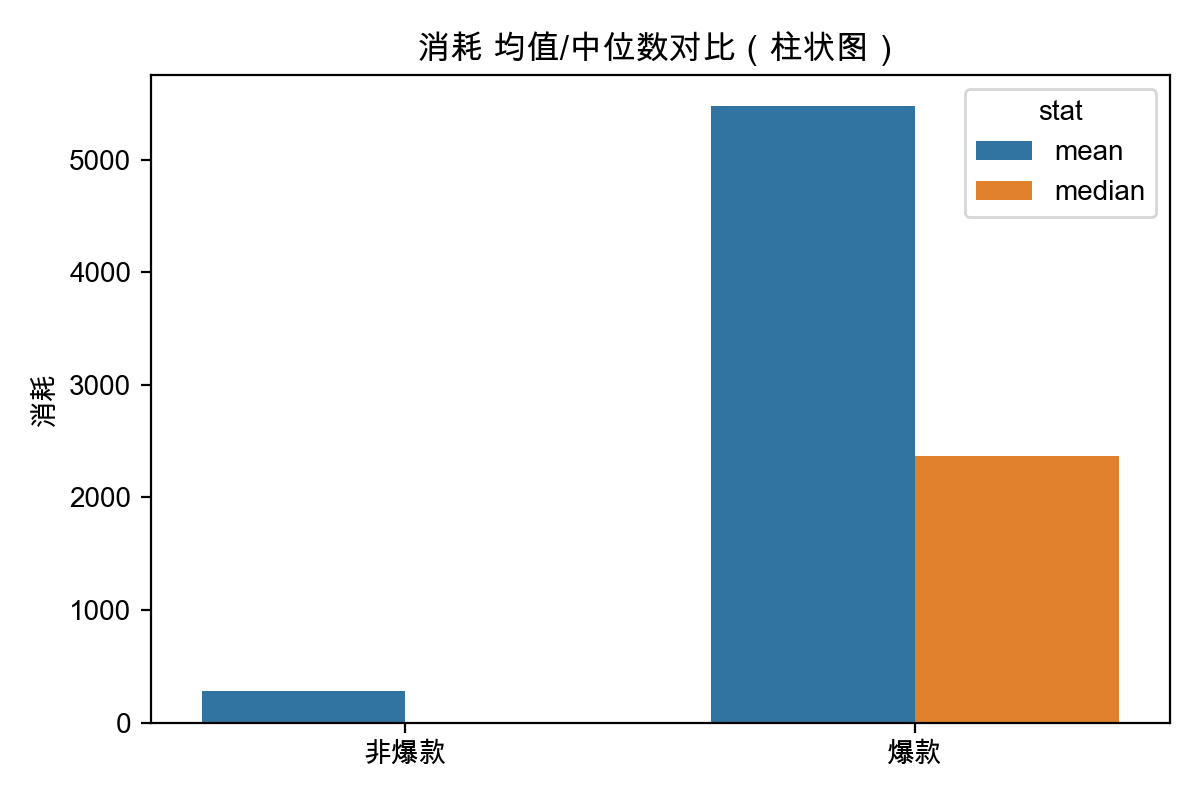
\includegraphics[width=\linewidth]{bar_metric_4ab855fb.png}
    \caption{柱状图（均值/中位数）}
  \end{subfigure}
  \caption{口径解释-消耗（规则内生指标）}
\end{figure}


\section{对现有分类合理性的初步思考与疑问}
\subsection{初步结论}
\begin{itemize}
  \item 从成交、播放、曝光、直播间行为等验证指标来看，爆款组显著优于非爆款组，现有分类与绩效表现总体相符。
  \item 由于爆款口径强调 高消耗 +点击率/转化率较高，当前标签更贴近 投放/流量分配 + 转化效率 的定义，未必等价于内容自然爆款（例如纯自然流量、互动驱动的爆款）。
\end{itemize}

\subsection{疑问与下一步建议}
\begin{itemize}
  \item 分层验证：下一步会按照\texttt{source}（dy/k7）分别计算同一套对比，检查结论是否一致。当前已经统计过分层统计表，可进一步补充分层图表。
  \item 指标口径：若业务上更关注 GMV，可进一步确认 直接成交金额/直接下单金额 是否可作为 GMV 代理，以及是否需要合并其它 GMV 字段。
  \item 长尾与零值：现在统计结果发现多个指标存在大量 0 值与长尾，如果这些值想要保留，后续报告可以更侧重中位数/分位数，并在图表中采用对数尺度或截尾展示。
  \item 内容侧解释：后续的研究思路是，把标题/标签/发布时间段等文本与时间特征纳入对比，解释为什么爆款更爆，而不仅是爆款更高。
\end{itemize}

\section{复现方式与产出清单}
\begin{itemize}
  \item 复现：运行 \texttt{Analysis/Week2\_Task3.ipynb}。将自动在 \texttt{Deliverables/week2\_task3/} 写出分析表、统计表与图表。
  \item 产出文件：
    \begin{itemize}
      \item \texttt{Deliverables/week2\_task3/K7直播间短视频分析表.xlsx}
      \item \texttt{Deliverables/week2\_task3/task3\_descriptive\_stats.xlsx}
      \item \texttt{Deliverables/week2\_task3/figures/*.png}
    \end{itemize}
\end{itemize}

\end{document}

